\documentclass[../main.tex]{subfiles}

\begin{document}
\section{Appendix}\label{sec:appendix}

\subsection{Auxiliary results}\label{sec:extraresults}

In this section, we present additional results that are referenced or utilized throughout the thesis. Due to their supporting nature, these results are included in the Appendix rather than in the main text.
  
Fix $k>2$ and recall that $G$ is the multiplicative group of coprime residue classes modulo $k$. Let $a>0$ and $r\geqslant 0$ be integers, and let $p$ be a prime. We say that $p^r$ \emph{precisely divides} $a$ if $p^r$ divides $a$ but $p^{r+1}$ does not. We then write $p^r\parallel a$. With this notation, the Chinese Remainder Theorem has the following implication.
\begin{lemma}\label{lem:Gbreaks}
	It holds that
	\begin{equation*}
		G\cong\prod_{p^r\parallel k}(\Z/p^r\Z)^\times,
	\end{equation*}
	where $p$ is a prime and $r\geqslant 0$ is a natural number.
\end{lemma}
\begin{proof}
	It is enough to note that every power $p^r$ precisely dividing $k$ will be relatively prime to any other, from which the result follows easily using the Chinese Remainder Theorem. 
\end{proof}
Therefore, the group $G$ breaks down as a direct product of abelian finite groups $(\Z/p^r\Z)^\times$, of order $\varphi(p^r)=(p-1)p^{r-1}$. This decomposition can be further expressed in terms of cyclic groups (which are unique up to isomorphism). If $p\neq 2$, the group $(\Z/p^r\Z)^\times$ is always cyclic. For $p=2$, the cases $r=1, 2$ are cyclic, but for $r\geqslant 3$ the group $(\Z/2^r\Z)^\times$ breaks down as a direct product of two cyclic groups. Specifically:
\begin{lemma}\label{lemma:cyclicgroups}
	Let $C_n$ denote the cyclic group of order $n\geqslant 1$. If $p$ is an odd prime and $r > 0$ is a natural number, then 
	\begin{equation}\label{eq:cyclicgroups1}
		(\Z/p^r\Z)^\times\cong C_{(p-1)p^{r-1}}.
	\end{equation}
	If $p=2$ and $r\geqslant 3$, then 
	\begin{equation}\label{eq:cyclicgroups2}
		(\Z/2^r\Z)^\times\cong C_2\times C_{2^{r-2}}.
	\end{equation}
	Moreover, $(\Z/2\Z)^\times\cong C_1$ and $(\Z/4\Z)^\times\cong C_2$, where we assume that $C_1$ is the trivial group.
\end{lemma}
\begin{proof}
	It is enough to prove that $(\Z/k\Z)^\times$ is a cyclic group if $k=2, 4$ or $k=p^r$, where $p$ is an odd prime and $r\geqslant 1$. This was first proved by Gauss, and a modern version can be found in \cite[Pages $61$, $62$ and $92$]{Shanks}. The case $k=2^r$ for $r\geqslant 3$ can be found in Gauss's original publication \cite{Gauss}.
\end{proof}

We now turn our attention to finding roots of a certain polynomial mod $p$. This will be relevant due to our \cref{def:Euclideanproof}. A useful tool to characterise the set of prime divisors of a polynomial of degree $2$ will be the so-called \emph{Quadratic Reciprocity Law} (QRL). Specifically, we are interested in giving conditions on the solutions of the equation $x^2-a \bmod{p}$, for some $a\in\Z$.

Let $p$ be a prime not dividing $a$. We say that $a$ is a \emph{quadratic residue} mod $p$ if there exists a solution to $x^2\equiv a\pmod{p}$. In other words,  $a$ is a quadratic residue mod $p$ if $a$ is a square mod $p$. Otherwise we say that $a$ is \emph{not a quadratic residue} mod $p$. With this language we can further define:
\begin{definition}
	Given $a\in\Z$ and $p$ an odd prime, the \emph{Legendre symbol} is defined by
	\begin{equation*}
		\legendre{a}{p}:=
		\begin{cases}
			0, & \text{if $p$ divides $a$}\\	
			1, & \text{if $a$ is a quadratic residue mod $p$}\\	
			-1, & \text{if $a$ is not a quadratic residue mod $p$.}\\	
		\end{cases}
	\end{equation*}
\end{definition}
The Legendre symbol has the following properties, which help us determine quadratic residues mod $p$, and are proved in \cite[Chapter 4]{Marcus}.
\begin{theorem}[\textbf{Gauss Quadratic Reciprocity Law}]\label{th:QR}
	Let $p$ and $q$ be two odd primes. Then, 
	\begin{equation}
		\legendre{p}{q}=(-1)^{\frac{p-1}{2}\frac{q-1}{2}}\legendre{q}{p}=
		\begin{cases}
			\legendre{q}{p}, & \text{if $p$ or $q \equiv 1\pmod{4}$}\\	
			-\legendre{q}{p}, & \text{if $p$ and $q \equiv 3\pmod{4}$.}\\	
		\end{cases}
	\end{equation}
	To this, there are two \emph{supplemental laws}:
	\begin{equation*}
		\legendre{-1}{p}=(-1)^{\frac{p-1}{2}}=
		\begin{cases}
			1, & \text{if $p \equiv 1\pmod{4}$}\\	
			-1, & \text{if $p \equiv 3\pmod{4}$}\\	
		\end{cases}
	\end{equation*}
	and
	\begin{equation*}
		\legendre{2}{p}=(-1)^{\frac{p^2-1}{8}}=
		\begin{cases}
			1, & \text{if $p \equiv 1$ or $ 7 \pmod{8}$}\\	
			-1, & \text{if $p \equiv 3$  or $5 \pmod{8}$.}\\	
		\end{cases}
	\end{equation*}	 
\end{theorem}

To finish this section, we turn our attention to the following property of Euler's phi function:

\begin{lemma}\label{lemma:propertyeulerphi}
	Let $m\geqslant 1$ and $n\geqslant 1$ be any integers. Then the equality $\varphi(nm)=\varphi(m)$ holds if and only if $n=1$ or $n=2$ and $m$ is odd.
\end{lemma}
\begin{proof}
	We may write
	\begin{equation*}
		m=2^s\prod_i p_i^{\alpha_i}\prod_j q_j^{\beta_j},
	\end{equation*}
	for some odd primes $p_i$, $q_j$ and some integers $s\geqslant 0$ and $\alpha_i,\beta_j \geqslant 1$. Similarly, we write
	\begin{equation}\label{eq:numbern}
		n=2^t\prod_j q_j^{\gamma_j}\prod_k r_k^{\delta_k},
	\end{equation}
	for some odd primes $r_k$ and some integers $t\geqslant 0$ and $\gamma_j,\delta_k\geqslant 1$. Observe that the primes $q_j$ are the common primes in the decomposition of $m$ and $n$ (with possibly different exponents $\beta_j$ and $\gamma_j$). Now, since Euler's function is multiplicative and supposing that $m$ is even ($s\geqslant 1$), we have
	\begin{equation*}
		\varphi(m)=2^{s-1}\prod_i(p_i-1)p_i^{\alpha_i-1}\prod_j(q_j-1)q_j^{\beta_j-1}
	\end{equation*}
	and 
	\begin{align*}
		\varphi(nm)&=2^{t+s-1}\prod_i(p_i-1)p_i^{\alpha_i-1}\prod_j(q_j-1)q_j^{\gamma_j+\beta_j-1}\prod_k(r_k-1)r_k^{\delta_k-1}\\
		&=2^{t+s-1}\prod_i(p_i-1)p_i^{\alpha_i-1}\prod_j(q_j-1)q_j^{\beta_j-1}\prod_jq_j^{\gamma_j}\prod_k(r_k-1)r_k^{\delta_k-1}.
	\end{align*}
	Imposing $\varphi(nm)=\varphi(m)$ and canceling terms we get
	\begin{equation*}
		2^t\prod_jq_j^{\gamma_j}\prod_k(r_k-1)r_k^{\delta_k-1}=1.
	\end{equation*}
	For the previous equality to hold, the term $\prod_k(r_k-1)r_k^{\delta_k-1}$ cannot appear, since $r_k$ are odd primes. Also, $t=0$ and $\gamma_j=0$ for every $j$. Therefore, from \cref{eq:numbern}, we deduce that $n=1$ if $m$ is even.
	
	However, if $m$ is odd ($s=0$) we have
	\begin{equation*}
		\varphi(m)=\prod_i(p_i-1)p_i^{\alpha_i-1}\prod_j(q_j-1)q_j^{\beta_j-1}
	\end{equation*}
	and
	\begin{align*}
		\varphi(nm)&=2^{t-1}\prod_i(p_i-1)p_i^{\alpha_i-1}\prod_j(q_j-1)q_j^{\gamma_j+\beta_j-1}\prod_k(r_k-1)r_k^{\delta_k-1}\\
		&=2^{t-1}\prod_i(p_i-1)p_i^{\alpha_i-1}\prod_j(q_j-1)q_j^{\beta_j-1}\prod_jq_j^{\gamma_j}\prod_k(r_k-1)r_k^{\delta_k-1}.
	\end{align*}
	Imposing $\varphi(nm)=\varphi(m)$ we get
	\begin{equation*}
		2^{t-1}\prod_jq_j^{\gamma_j}\prod_k(r_k-1)r_k^{\delta_k-1}=1.
	\end{equation*}
	For the previous equality to hold, the term $\prod_k(r_k-1)r_k^{\delta_k-1}$ cannot appear, since $r_k$ are odd primes. Also, $t=1$ and $\gamma_j=0$ for every $j$. Therefore, from \cref{eq:numbern}, we deduce that $n=2$ if $m$ is odd.
\end{proof}

We have duplicate labels for some cyclotomic fields: if we let $\zeta_n$ denote an $n$th primitive root of unity, we have $\Q(\zeta_{2m})=\Q(\zeta_{m})$ if $m$ is odd. This is the only case two different labels describe the same field in light of \cref{lemma:propertyeulerphi}. Thus, when dealing with the cyclotomic field $\Q(\zeta_n)$, it is common to require $n$ is not twice an odd number, that is, $n\not\equiv 2\pmod{4}$.

\subsection{Natural and Dirichlet Density}\label{sec:naturalDirichletdens}
We have seen in \cref{sec:Chebotarev} that, in order to accurately use Chebotarev Density Theorem, one needs to define a measure for sets of primes (or prime ideals). The most natural way to construct a density of a given set of primes is as follows.

Let $\Pi$ be the set of all prime numbers. Let $S\subseteq\Pi$ be a subset and let $p$ be a prime. For any real number $x\geqslant 1$, we define the \emph{upper natural density} and the \emph{lower natural density} of $S$ in $\Pi$ as
	\begin{equation*}
		\limsup_{x\rightarrow\infty}\frac{\#\{p\in S: p < x\}}{\#\{p\in \Pi: p < x\}}, \quad \liminf_{x\rightarrow\infty}\frac{\#\{p\in S: p < x\}}{\#\{p\in \Pi: p < x\}},
	\end{equation*}
	respectively. If both these densities coincide, we call the common value the \emph{natural density} (or \emph{asymptotic density}) of $S$ in $\Pi$, and we write it as
	\begin{equation*}
		\delta(S):=\lim_{x\rightarrow\infty}\frac{\#\{p\in S: p < x\}}{\#\{p\in \Pi: p < x\}}.
	\end{equation*}
Many properties we would expect are in fact true: if $S$ does have a density, then $0\leqslant \delta(S)\leqslant 1$, since $\delta(\Pi)=1$. Also, given that $\Pi$ is infinite, any finite set of primes will have density equal to $0$.

A less restrictive (yet less intuitive) notion of density is obtained via Dirichlet series. Recall that $\sum_{p\in\Pi}p^{-1}$ is divergent, and again let $S\subseteq\Pi$ be a subset. We define the \emph{upper Dirichlet density} and the \emph{lower Dirichlet density} of $S$ in $\Pi$ as
	\begin{equation*}
		\limsup_{s\rightarrow 1^+}\frac{\sum_{p\in S}p^{-s}}{\sum_{p\in \Pi}p^{-s}}, \quad \liminf_{s\rightarrow 1^+}\frac{\sum_{p\in S}p^{-s}}{\sum_{p\in \Pi}p^{-s}},
	\end{equation*}
	respectively. If both these densities coincide, we call the common value the \emph{Dirichlet density} (or \emph{analytic density}) of $S$ in $\Pi$, and we write it as
	\begin{equation}\label{eq:Dirichletdensity}
		d(S):=\lim_{s\rightarrow1^+}\frac{\sum_{p\in S}p^{-s}}{\sum_{p\in \Pi}p^{-s}}.
	\end{equation}

The Dirichlet density in \cref{eq:Dirichletdensity} can be expressed in a more convenient way. Recall that Euler discovered the following relation between the Riemann zeta function and prime numbers\footnote{Here $\zeta(s)$ denotes the Riemann zeta function, not a $k$th root of unity.}:
\begin{equation}\label{eq:Riemannzeta}
	\zeta(s)=\sum_{n=1}^{\infty}\frac{1}{n^s}=\prod_{p\in \Pi}\frac{1}{1-p^{-s}},
\end{equation}
for any complex number $s$ with $\Re(s)>1$. Using the formula for the sum of a geometric progression we can further write
\begin{equation*}
	\zeta(s)=\prod_{p\in \Pi}\sum_{n=0}^{\infty}p^{-ns},
\end{equation*}
since $\abs{p^{-s}}=p^{-\Re(s)}<1$. Now, $\zeta(s)$ has a single pole of order $1$ at $s=1$, so we have that, letting $s\rightarrow1^+$
\begin{equation}\label{eq:Riemannzeta2}
	(s-1)\sum_{n=1}^{\infty}\frac{1}{n^s}=(s-1)\zeta(s)=1+o(1).
\end{equation} 
Taking the logarithm from \cref{eq:Riemannzeta2} and using \cref{eq:Riemannzeta} we can write
\begin{equation}\label{eq:Riemannzeta3}
	O(1)=\log(s-1)+\log\zeta(s)=\log(s-1)+\sum_{p\in \Pi}\log(\frac{1}{1-p^{-s}}).
\end{equation}

Now, since $\abs{p^{-s}}<1$ and $p^{-s}\neq 1$, a Taylor expansion yields
\begin{equation*}
	\sum_{p\in \Pi}-\log(1-p^{-s})=\sum_{p\in \Pi}\sum_{n=1}^{\infty}\frac{p^{-ns}}{n}\leqslant \sum_{p\in \Pi}\sum_{n=1}^{\infty}p^{-ns}.
\end{equation*}
Since the sum $\sum_{n=1}^{\infty}p^{-ns}$ converges, we can write 
 \begin{equation*}
 	\sum_{p\in \Pi}-\log(1-p^{-s})=C\sum_{p\in \Pi}\sum_{n=1}^{\infty}p^{-ns}
 \end{equation*}
for some constant $C>0$ and absorb it to write \cref{eq:Riemannzeta3} as
\begin{equation}\label{eq:O1}
	O(1)=\log(s-1)+\sum_{p\in \Pi}\sum_{n=1}^{\infty}p^{-ns}.
\end{equation}
Since the last sum converges absolutely because $\Re(s)>1$, we can write
\begin{equation}\label{eq:O1_2}
\sum_{p\in \Pi}\sum_{n=1}^{\infty}p^{-ns}=\sum_{p\in \Pi}p^{-s}+\sum_{p\in \Pi}\sum_{n=2}^{\infty}p^{-ns}.
\end{equation}

We will now see that, in fact, 
\begin{equation}\label{eq:sum_goal}
	\sum_{p\in \Pi}\sum_{n=2}^{\infty}p^{-ns}=O(1).
\end{equation}
To show this equality, start by noting that
\begin{equation*}
	\sum_{n=2}^{\infty}p^{-ns}=\frac{p^{-2s}}{1-p^{-s}}.
\end{equation*}
Also, letting $\sigma:=\Re(s)>1$ and observing that $\abs{p^{-s}}=p^{-\sigma}<1$, we have
\begin{equation*}
	\abs{\frac{p^{-2s}}{1-p^{-s}}}\leqslant \frac{p^{-2\sigma}}{1-p^{-\sigma}}\leqslant p^{-2\sigma}C_\sigma,
\end{equation*}
for some constant $C_\sigma>0$ depending on $\sigma$, so the left-hand side of \cref{eq:sum_goal} is bounded by
\begin{equation}\label{eq:Riemannzeta4}
	\sum_{p\in \Pi}\sum_{n=2}^{\infty}p^{-ns} \leqslant \sum_{p\in \Pi}\frac{p^{-2\sigma}}{1-p^{-\sigma}}\leqslant \sum_{p\in \Pi}\frac{C_\sigma}{p^{2\sigma}}.
\end{equation}
It is now enough to remember that for $\sigma>1$, 
\begin{equation*}
	\sum_{p\in \Pi}\frac{1}{p^{2\sigma}}<\infty,
\end{equation*}
so, from \cref{eq:Riemannzeta4}, we finally have
\begin{equation*}
	\sum_{p\in \Pi}\sum_{n=2}^{\infty}p^{-ns} \leqslant C_\sigma\sum_{p\in \Pi}\frac{1}{p^{2\sigma}}<\infty.
\end{equation*} 

Putting \cref{eq:O1_2} and \cref{eq:sum_goal} together, we can write \cref{eq:O1} as
\begin{equation*}
	\sum_{p\in \Pi}p^{-s}=-\log(s-1)+O(1),
\end{equation*}
so, observing \cref{eq:Dirichletdensity}, the Dirichlet density of $S$ is given by 
\begin{equation}\label{eq:Dirichletdensfinal}
	\lim_{s\rightarrow1^+}\frac{\sum_{p\in S}p^{-s}}{-\log(s-1)}
\end{equation}
if the limit exists. 

It can be shown that the Dirichlet density is a generalisation of the natural density: if the natural density exists, then the Dirichlet density also exists, and they both coincide. However, the converse assertion is not always true. There is an example due to Enrico Bombieri (referenced in \cite{Serre}) that shows this case. If $P^1$ is the set of prime numbers whose first digit is equal to one, then $P^1$ does not have a natural density, but its Dirichlet density does exist and equals $d(P^1)=\log_{10}2\approx0.30102999566$.

 It is natural to extend \cref{eq:Dirichletdensfinal} to sets of prime \emph{ideals}. Let $\mathfrak{p}$ be some prime ideal lying above $p$ with $\Norm(\mathfrak{p})=p^f$ for some inertia degree $f$. The generalisation is accomplished through the same procedure we have outlined above, instead using the \emph{Dedekind zeta function}.
  
Let $K$ be a number field and again let $s\in \C$ with $\Re(s)>1$. The \emph{Dedekind zeta function} $\zeta_K(s)$ is a function in the complex plane given by
	\begin{equation}\label{eq:Dedekindzeta}
		\zeta_K(s):=\sum_{\mathfrak{a}\subseteq\mathcal{O}_K}\frac{1}{\Norm(\mathfrak{a})^{s}}=\prod_{\mathfrak{p}\subseteq\mathcal{O}_K}\frac{1}{1-\Norm(\mathfrak{p})^{-s}},
	\end{equation}
	where $\mathfrak{a}$ ranges over the non-zero ideals of $\mathcal{O}_K$ and $\mathfrak{p}$ ranges over the non-zero prime ideals of $\mathcal{O}_K$. Dedekind zeta function has only one pole, which is simple, at $s=1$. In the case $K=\Q$, \cref{eq:Dedekindzeta} trivially reduces to the Riemann zeta function.

\subsection{Schur Theorem hypothesis}\label{sec:thhypothesis}
Recall that to prove that there are infinitely many primes $\equiv\ell\pmod{k}$ if $\ell^2\equiv 1\pmod{k}$ we strongly use the fact that there exists at least one prime $\equiv\ell\pmod{k}$. In particular, the argument in \cref{th:infiniteprimes} requires the existence of one such prime, and so it is needed in the automated proof if $\ell\not\equiv 1 \pmod{k}$ (see \cref{sec:generalproof}). Affirming that such a prime exists for every $k$ and $\ell$ relatively prime requires advanced mathematics. In fact, if we assume this claim to be true, Dirichlet \cref{th:Dirichlet} follows easily: we would just need the Chinese Remainder Theorem to obtain Dirichlet's well-known result.
\begin{lemma}
	Suppose that $k$ and $\ell$ are two fixed, non-zero integers satisfying $\gcd(k, \ell)=1$. Also suppose that for every such $k$ and $\ell$ there exists a prime $p$ that is $\equiv\ell\pmod{k}$. Then, there are infinitely many primes $\equiv\ell\pmod{k}$.
\end{lemma}
\begin{proof}
	By hypothesis, there exists a prime $p_1\equiv \ell\pmod{k}$. Now, since 
	\begin{equation*}
	\gcd(k, p_1)=\gcd(k, kn_1+\ell)=\gcd(k,\ell)=1, 
	\end{equation*}
	for some $n_1\in\Z$, the Chinese Remainder Theorem guarantees the existence of $\ell_1\in\Z$, which is a solution to the system
	 	\begin{equation}\label{eq:cases-1}
	 	\begin{cases}      
	 		\ell_1\equiv \ell \pmod{k}\\
	 		\ell_1\equiv 1 \pmod{p_1}.
	 	\end{cases}
	 \end{equation}
	 
	 Now observe that $k_1:=kp_1$ and $\ell_1$ satisfy the hypothesis of the lemma. Indeed, for some integer $m_1$ we have:
	 \begin{equation*}
	 	\gcd(k_1,\ell_1)=\gcd(kp_1,\ell_1)=\gcd(k,\ell_1)\gcd(p_1,\ell_1)=\gcd(k,km_1+\ell)\cdot 1=1\cdot 1=1,
	 \end{equation*}
	 where we have used well-known properties of the greatest common divisor, the first equality in \cref{eq:cases-1} to write $\ell_1=km_1+\ell$, and the second one to deduce that $\gcd(p_1,\ell_1)=1$. Thus, there exists one prime $p_2\equiv\ell_1\pmod{k_1}$. Observe that $p_2\equiv\ell\pmod{k}$, using the first equation in \cref{eq:cases-1}, and $p_2\equiv 1\pmod{p_1}$ using the second one (this last condition shows that $p_2\neq p_1$). We could now start the argument once again. Suppose we have a prime $p_i\equiv\ell\pmod{k}$ for $i\geqslant 2$. Again, 
	 \begin{equation*}
	 	\gcd(k,p_i)=\gcd(k,kn_i+\ell)=\gcd(k,\ell)=1,
	 \end{equation*}
	 for some $n_i\in \Z$, so there exists $\ell_i\in \Z$ which is a solution to the system
	 	\begin{equation}\label{eq:cases-2}
	 	\begin{cases}      
	 		\ell_i\equiv \ell \pmod{k}\\
	 		\ell_i\equiv 1 \pmod{p_i},
	 	\end{cases}
	 \end{equation}
	and one can find a new prime $\equiv\ell\pmod{k}$ considering $k_i:=kp_i$ and $\ell_i$ for $i\geqslant 2$. We have
	 \begin{equation*}
	 	\gcd(k_i,\ell_i)=\gcd(kp_i,\ell_i)=\gcd(k,\ell_i)\gcd(p_i,\ell_i)=\gcd(k,km_i+\ell)\cdot 1=1\cdot 1=1,
	 \end{equation*}
	where we have used again \cref{eq:cases-2}. Thus, there exists a prime $p_{i+1}\equiv\ell_i\pmod{k_i}$, and again $p_{i+1}\equiv\ell\pmod{k}$ and $p_{i+1}\equiv1\pmod{p_i}$, so $p_{i+1}$ is yet a new prime $\equiv\ell\pmod{k}$ different from $p_i$. In this way, infinitely many primes $\equiv \ell \pmod{k}$ can be constructed.
\end{proof}

No proof using elementary techniques is known of the fact that there exists one prime $\equiv\ell{\pmod{k}}$ for every $k$ and $\ell$, so this needs to be a hypothesis of \cref{th:infiniteprimes}.


\subsection{Small cases}\label{sec:smallcases}
The automated proofs for the cases $k=1,2,3,4,6$ are treated separately, since they are degenerate cases and deserve a special (and somewhat easier) treatment.

\subsubsection{Case \texorpdfstring{$k=1, 2$}{k=1,2}}
In these cases, we can only consider $\ell=1$ and the extension $\Q(\zeta)/ \Q$ collapses because $\degpol(\Phi_k)=1$, causing $\Q(\zeta)=\Q$. In these cases, a Euclidean proof can be easily established. In fact, the case $k=1$ follows directly from Euclid \cref{th:Euclid}. The case $k=2$ and $\ell=1$ reads as follows:
\begin{lemma}
	There are infinitely many primes $\equiv 1\pmod{2}$.
\end{lemma}
\begin{proof}
Suppose there are finitely many primes $\equiv 1 \Mod{2}$, say $p_1, p_2,\dots,p_m$. Our goal is to show that there exists yet another prime $\equiv 1 \Mod{2}$ not in our list. For this goal, consider $Q:=p_1p_2\cdots p_m$ and the polynomial $f(x):=2x-1$. Now, $f(Q) = 2p_1p_2\cdots p_m-1=2Q-1$. This number has at least one prime divisor, $p$, since it is greater than one. We then have that $p$ divides $2Q-1$.

Next, observe that $p\neq p_i$ for every $i$ such that $1\leqslant i \leqslant m$: if $p=p_i$ for some $i$, then $p$ would divide $2Q$. Since $p$ also divides $2Q-1$, we get that $p$ divides $1$, so $p=1$, which is a contradiction ($1$ is not a prime). Therefore, $p$ is a prime divisor of $2Q-1$ not in our list. Finally, note that $2Q-1$ has all its prime divisors $\equiv 1 \Mod{2}$ since it is odd, so $p$ is a new prime $\equiv 1 \pmod{2}$.

This gives us an infinitude of primes $\equiv 1 \Mod{2}$ provided we have one. Since $3$ is a prime $\equiv 1 \Mod{2}$, the desired result is finally settled.
\end{proof}
The case $k=2$ is the only case where the Euclidean polynomial considered for the proof is not monic. However, $f(x)=2x-1$ satisfies every other condition in the definition of Euclidean polynomial in \cref{sec:fundamentals}, and it clearly follows the spirit of Euclid Theorem.

\subsubsection{Case \texorpdfstring{$k=3, 4, 6$}{k=3,4,6}}
In these cases, $\degpol(\Phi_k)=\varphi(k)=\abs{G}=2$, which leads to $G=H$ in the case $\ell\not\equiv 1 \pmod{k}$. We will consider the same polynomial $f_u(x)$ of \cref{prop:fuirreducible}, but it will now be easy to justify the prime divisors of this polynomial\footnote{Since we have already chosen the integer $u$ in $f_u$ to satisfy \cref{lemma:integervalcyclo}, we shall write $f$ instead of $f_u$.}. We just have to note that every prime divisor $p$ of $f$ has to be, in particular, a prime, and that rules out many options. For the case $k=3$, this means that $p\equiv 1,2 \pmod{3}$ (or $p=3$); for $k=4$, $p\equiv 1,3 \pmod{4}$ (or $p=2$); and for $k=6$, $p\equiv 1,5 \pmod{6}$ (or $p=2,3$).

Therefore, the proof for the cases $\equiv 2 \pmod{3}$, $\equiv 3 \pmod{4}$, and $\equiv 5 \pmod{6}$ can be easily handled using only the contradiction argument at the end of \cref{th:infiniteprimes}, as \cref{th:fdivisors} is not necessary to work out the prime divisors of $f$. To see how the automatic proofs look in these cases, use the webpage link\footnote{Access \url{http://167.172.185.115} to visit the webpage.}.

The cases $\equiv 1\pmod{k}$ are trickier, since we have to show that every prime $p$ that divides $f$ satisfies $p\equiv 1 \pmod{k}$ (except finitely many cases). In fact, every possible value of $k$ (except for $k=1,2$) requires the same treatment when dealing with the case $\equiv 1\pmod{k}$. This is already fully described in \cref{sec:generallcong1}.

\subsection{Automated proofs' code}\label{sec:code1}
The automated proofs are generated with a combination of SageMath and \LaTeX. Roughly speaking, the SageMath code\footnote{The code developed can be entirely found in the Git repository \url{https://github.com/joarca01/final-math-bsc-thesis}.} generates the necessary calculations for the specific values of $k$ and $\ell$, calling various templates to write the necessary quantities in predefined spaces in the final \LaTeX \ file containing the proof. 

Specifically, the main function in our code is called \textcolor{blue}{\textmyfont{ap\_euc}} (which stands for ``Arithmetic Progression Euclidean''), and it only takes two arguments, $k$ and $\ell$. After some steps, it writes a \LaTeX \ file with the proof for the selected arithmetic progression univocally defined by these two parameters. This is achieved through the following (simplified) steps:
\begin{enumerate}
	\item First, the supplied values of $k$ and $\ell$ are checked to ensure they are positive integers, satisfying $\gcd(k, \ell)=1$, $\ell^2\equiv 1 \pmod{k}$, and $k>\ell$. These are, in fact, the same constraints we imposed at the beginning of \cref{sec:fundamentals}. If any of these conditions is not met, the execution stops and an error arises.
	\item If $k=1,2$ the code points to a file named \texttt{proof\_1\_mod1.tex} or \texttt{proof\_1\_mod2.tex}, where the proofs for the cases $\equiv 1 \pmod{1}$ and $\equiv 1 \pmod{2}$ are respectively found. No code is used for these two cases, since they are degenerate, and their proof has been written manually, with a very simple Euclidean argument. The function \textcolor{blue}{\textmyfont{ap\_euc}} returns here in these cases.
	\item Next, an empty dictionary is initialized, where every value, polynomial, sentence, or character that will appear in the final proof is stored. A different key is given to each variable. As an example, the values $k$ and $\ell$ are saved under the keys ``k'' and ``ell'' in the dictionary, while the coprime integers to $k$ are calculated with the function \textcolor{blue}{\textmyfont{coprimes}} (which is called from the auxiliary file \texttt{utils.ipynb}) and assigned to the key ``coprimes\_list''. Every function we call is either defined in this auxiliary file\footnote{Access the Git Repository to view the exact code of every function we created in the file \texttt{utils.ipynb}.} or is a built-in SageMath function. Some variables (like the ``factored\_k'' below) are not included in the dictionary because they are needed for future calculations but are not directly included in the final \LaTeX \ file.\\
	
	\begin{python}
		
		d['k'] = k
		d['ell'] = l
		d['coprimes_list'] = coprimes(k)
		factored_k = ZZ(k).factor(proof=False)
		primes_div_k_list = prime_divisors(factored_k)
		d['sufix_cyclo_alt'] = sufix_cyclo(k) # Contains the string    'st', 'nd' or 'rd'.
		d['eulersphi_k'] = euler_phi(k) # Contains Euler totient function value at k.
	\end{python}
	
	Note that the variables that are lists have their key ending with ``\_list''. This will be necessary for a correct displaying of lists in the final \LaTeX \ document.
	\item Then, the file takes two different routes if $\ell\equiv 1\pmod{k}$ or else. The first case is slightly simpler.
	\item The code again splits between the cases $k=3,4,6$ and every other value of $k$. In this part of the code, the prime divisors of $f$ must be justified. In the cases $k=3,4,6$, this can be easily done with one sentence, which is stored in a \LaTeX \ file, which we call \texttt{template3\_alt.tex}. This template is then read in the main function and assigned to the dictionary key ``prime\_divisors\_argument\_alt'' as follows.\\
	
	\begin{python}
		
		if k == 3 or k == 4 or k == 6:
		
		template3_alt = Path('template3_alt.tex').read_text()
		d['prime_divisors_argument_alt'] = subst_dictionary(template3_alt,d)
	\end{python}
	
	The cases $k=3,4,6$ now go directly to the end of the function (corresponding to the last item of this list). In every other possible value of $k$, the justification of the prime divisors of $f$ is considerably longer. As before, a template stores a sentence stating that the proof of the form of every prime divisor of $f$ will be given later on in the document.
	
	\item The whole code is written so it can overcome a possible stall of the factorization of $\Delta(f)$ or $f(0)$, as described in \cref{sec:programlimit} and \cref{sec:altarguments}. Whenever a factorization has to be made, it is encapsulated in a ``try/except Runtime Error'' clause. The factorization is first tried in the ``try''. If it fails in the specified time threshold of $2$ seconds, the code jumps to the ``except RuntimeError'' part, where an alternative argument is instead written in the corresponding variables. The function we use to factor any quantity is the following:\\
	
	\begin{python}
		
		def factor_timeout(n, timeout = 2):
		with stopit.ThreadingTimeout(timeout) as to_ctx_mgr: 
		ans = fork(lambda n: ZZ(n).factor(), timeout = timeout)(n)
		return ans
		if to_ctx_mgr.state in [to_ctx_mgr.TIMED_OUT, to_ctx_mgr.INTERRUPTED]:
		print('The factorization takes too long.')
		raise RuntimeError
	\end{python}
	
	\item It is worth showing the code of the \textcolor{blue}{\textmyfont{subst\_dictionary}} function, which substitutes the values of the dictionary into a given \LaTeX \ document. This function separates the cases where the value of the key is a list or the key ends with ``\_alt'' from every other case. This is done to ensure that the value is correctly displayed in the final document.\\
	
	\begin{python}
		
	def subst_dictionary(template, dictionary):
		for ky, val in dictionary.items():
			if type(val) == list: # Remove the square brackets if val is a Python list.
				template = template.replace(f'{{{ky}}}', str(latex(val))[6:-7]) 
			if ky[-3:] == "alt":
				template = template.replace(f'{{{ky}}}', val)
			else:
				template = template.replace(f'{{{ky}}}', latex(val))
		return template
	\end{python}
	
	\item Finally, the proof is written in the file \texttt{template\_euc.tex} (or \texttt{template\_lcong1\_euc.tex} in the case $\ell\equiv 1\pmod{k}$). The function \textcolor{blue}{\textmyfont{subst\_dictionary}} above writes every dictionary key in its predefined position in the template. Lastly, a file called \texttt{proof\_euc.tex} (or  \texttt{proof\_lcong1\_euc.tex}) is created, which finally contains the proof of the infinitude of primes $\equiv\ell\pmod{k}$. 
	
 	This definitive file is saved in the current user path where the function \textcolor{blue}{\textmyfont{ap\_euc}} has been called. This \LaTeX \ file is then converted to HTML source and inserted in the webpage.\\
	
	\begin{python}
		
		template = Path('template_euc.tex').read_text()
		output = subst_dictionary(template,d)
		
		with open('proof_euc.tex','w') as f:
			f.write(output)
	
		return 
	\end{python}
	
\end{enumerate}

\subsection{Murty's example}\label{sec:MurtysExample}

Taking into account all the theorems and ideas we have developed, our version of the Euclidean proof in \cref{sec:generalproof} seems the most reasonable. However, in Murty's article \cite{Murty}, which is the reference we have mostly followed, no example with specific values of $k$ and $\ell$ is given to the extent that we have. Instead, the author makes use of the Quadratic Reciprocity Law (QRL) to provide a brief proof of the infinitude of primes $\equiv 4\pmod{15}$. However, not every pair of $k$ and $\ell$ satisfying $\ell^2\equiv 1 \pmod{k}$ admits such a proof. It can be checked (see the discussion following \cref{prop:Murtyexample} below) that a proof using the QRL will only work when $L=\Q(\eta)$ is the compositum of its quadratic subfields\footnote{A \emph{quadratic extension} of $\Q$ is of the form $\Q(\sqrt{D})$, where $D\in\Z$ is square-free.}, which is not always the case (recall \cref{prop:fuirreducible}). While significantly shorter, the proof using the QRL does not cover every possible arithmetic progression satisfying Schur and Murty's condition, so we have chosen not to automatize this approach.

For completeness, we shall reproduce (and improve) Murty's proof for the specific case $k=15$ and $\ell=4$ and later explain why his argument is not always possible.

\begin{proposition}\label{prop:Murtyexample}
	There exist infinitely many primes $\equiv 4\pmod{15}$.
\end{proposition}
\begin{proof}
	Consider the polynomial
	\begin{equation*}
		f(x):=\big(x-(\zeta+\zeta^4)\big)\big(x-(\zeta^2+\zeta^8)\big)\big(x-(\zeta^7+\zeta^{13})\big)(x-(\zeta^{11}+\zeta^{14})\big),
	\end{equation*}
	where $\zeta=e^{2\pi i/15}$ is a $15$th primitive root of unity. Simplifying leads to $f(x)=x^4-x^3+2x^2+x+1$.
	
	Now, write $f$ as $f(x)=(-x^2+x/2-1/2)^2+3(x+1)^2/4$. Suppose $p$ is a prime divisor of $f$. Thus, for some $n\in \Z$ it is true that
	\begin{equation*}
		\bigg(-n^2+\frac{n}{2}-\frac{1}{2}\bigg)^2+\frac{3(n+1)^2}{4}\equiv0 \pmod{p} \Rightarrow -3 \equiv \Bigg(\frac{-n^2+n/2-1/2}{(n+1)/2}\Bigg)^2 \pmod{p},
	\end{equation*}
	which is of the form $m^2+3=pm'$ for some non-zero integers $m$ and $m'$ (if $p\neq3$). Therefore, $-3$ is a quadratic residue for every prime divisor of $f$ unequal to $3$, so $\legendre{-3}{p}=-1$. By the Legendre symbol's properties, $\legendre{-3}{p}=\legendre{p}{3}=1$, which happens if and only if $p\equiv 1\pmod{3}$. 
	
	If we instead write $f$ as $f(x)=(-x^2+x/2-3/2)^2-5(x-1)^2/4$ ---and follow the same reasoning as before--- we deduce that any prime divisor of $f$ unequal to $5$ satisfies $\legendre{5}{p}=\legendre{p}{5}=1$, which happens if and only if $p\equiv 1$ or $4 \pmod{5}$.
	
	With these two conditions over $p$, we deduce that any prime divisor of $f$ is either $\equiv 1$ or $4 \pmod{15}$, except for $p=2,3,5$. (Note that the prime $2$ is added since it is never considered in the definition of the Legendre symbol). By \cref{lemma:propertiesprimedivisors2}, the polynomial $f(15x+1)$ also has its prime divisors $\equiv 1$ or $4 \pmod{15}$ except for $p=2,3,5$. A Taylor expansion yields:
	\begin{equation*}
		f(1+15x)=f(1)+f'(1)15x+O((15x)^2)=4+6\cdot15x+O((15x)^2)=15xg(x)+4,
	\end{equation*} 
	for some $g\in\Z[x]$. To reach a contradiction, suppose that there is a finite number of primes $\equiv 4\pmod{15}$, and let $Q$ be their product. Now, consider $f(1+15Q)=15Qg(Q)+4$. We will first show that this number has no prime divisors $\equiv 4 \pmod{15}$. If we suppose otherwise, let $q$ be a prime such that $q$ divides $15Qg(Q)+4$ and $q\equiv 4 \pmod{15}$. Observe that $q$ divides $Q$ by definition, so $q$ also divides $15Qg(Q)$. Then, it follows that $q$ divides $4$, so it must happen that $q=2$, which is a contradiction since then $q\not\equiv 4 \pmod{15}$. 
	
	Therefore,  $f(1+15Q)=15Qg(Q)+4$ has no prime divisors $\equiv 4 \pmod{15}$. Furthermore, $2, 3$ and $5$ are also not prime divisors of $f(1+15Q)$. Indeed,
	\begin{equation*}
		f(1+15Q)\equiv f(1)=4 \pmod{15},
	\end{equation*}
	so $f(1+15Q)$ is not divisible by $3$ or $5$. Similarly, observing that $Q$ is odd since it is a product of primes excluding $2\not\equiv 4 \pmod{15}$,
	\begin{equation*}
		f(1+15Q)\equiv f(1+1)\equiv f(0)=1 \pmod{2},
	\end{equation*}
	so $f(1+15Q)$ is not divisible by $2$. 
	
	Since every prime divisor of $f$ is either $\equiv 1$ or $4\pmod{15}$ or $2,3,5$, it follows that every prime divisor of $f(1+15Q)$ must be $\equiv 1 \pmod{15}$. Therefore, $f(1+15Q)\equiv 1 \pmod{15}$. However, $f(1+15Q)=15Qg(Q)+4\equiv 4 \pmod{15}$. This is a contradiction. Therefore, there exist infinitely many primes $\equiv 4 \pmod{15}$.
\end{proof}

	The key to the previous theorem is characterising the prime divisors of $f$. This is achieved via studying these prime divisors in each of the quadratic subfields of $L=\Q(\eta)$ with $\eta=h_{15}(\zeta)=(\zeta-15)(15-\zeta^4)=-\zeta^5+15\zeta^4+15\zeta-225$, which are $F_1=\Q(\sqrt{-3})$, $F_2=\Q(\sqrt{5})$ and $F_3=\Q(\sqrt{-15})$. This is acceptable since $L$ coincides with the compositum $F_1F_2F_3$. In this case, studying the prime divisors of $f$ in every $F_i$ is equivalent to studying them in $L$. Since $[F_i:\Q]=2$ for every $i$, the QRL effectively gives a characterisation in terms of congruences of these prime divisors (in each quadratic subfield). 
	
	Nevertheless, it is not true in general that $L$ is the compositum of its quadratic subfields. Since reciprocity laws of higher order are not in general easy to express via congruences (unless $L$ is a cyclotomic field or quadratic over $\Q$), the argument in \cref{prop:Murtyexample} does not work for every arithmetic progression satisfying $\ell^2\equiv 1\pmod{k}$. 
	
	Also, observe that the proof in \cref{prop:Murtyexample} has both some similarities and some differences with our general Euclidean method. Starting with the similarities, our Euclidean polynomial $f^*$ defined in \cref{sec:theoretical} for the progression $\equiv 4\pmod{15}$ has the same degree and prime divisors as the polynomial $f$ in  \cref{prop:Murtyexample} (despite being significantly different in their coefficients\footnote{For the progression $\equiv 4 \pmod{15}$, our general method produces the polynomial $f^*(x)=x^{4} + 883 x^{3} + 292728 x^{2} + 43186723 x + 2392743361$.}). Indeed, in Murty's proof, we have seen that the prime divisors $p$ of $f$ satisfy $p\equiv 1, 4 \pmod{15}$ or $p=2, 3, 5$, and the prime divisors of $f^*$, because of \cref{th:fdivisors}, are also those primes $\equiv 1, 4 \pmod{15}$, together with the prime divisors of $15$ and $\Delta(f^*)=900=2^2\cdot3^2\cdot5^2$, which are $2, 3$ and $5$. Thus, $f$ also satisfies our definition of Euclidean polynomial.
	
	With respect to the differences, observe that the polynomial $f^*$ is the minimal polynomial of $\eta\in L$. Also, $f^*$ generates the field $L$, and its special properties (see \cref{lemma:integervalcyclo} for example) help us build the Euclidean proof in general. All these constraints on $f^*$ make it a complex polynomial in its coefficients. However, for the specific case proved above, we do not need $f$ to be the minimal polynomial of any element of $L$. We just want it to generate $L$ and have the right prime divisors. There are multiple polynomials that accomplish this, and Murty has chosen the simplest one in its coefficients, which is the irreducible polynomial $f(x)=x^4-x^3+2x^2+x+1$. Nevertheless, this polynomial does not follow directly from the construction Murty gives in his article.

\subsection{Program's execution time}\label{sec:exectime}

Find below the figures that show the performance of our code that yields the proof of the infinitude of primes $\equiv\ell\pmod{k}$, in the cases $k\in[20,80]$, with $\ell$ such that $\ell^2\equiv 1\pmod{k}$.

\begin{sidewaysfigure}
	\centering
	\vspace*{-3in}
	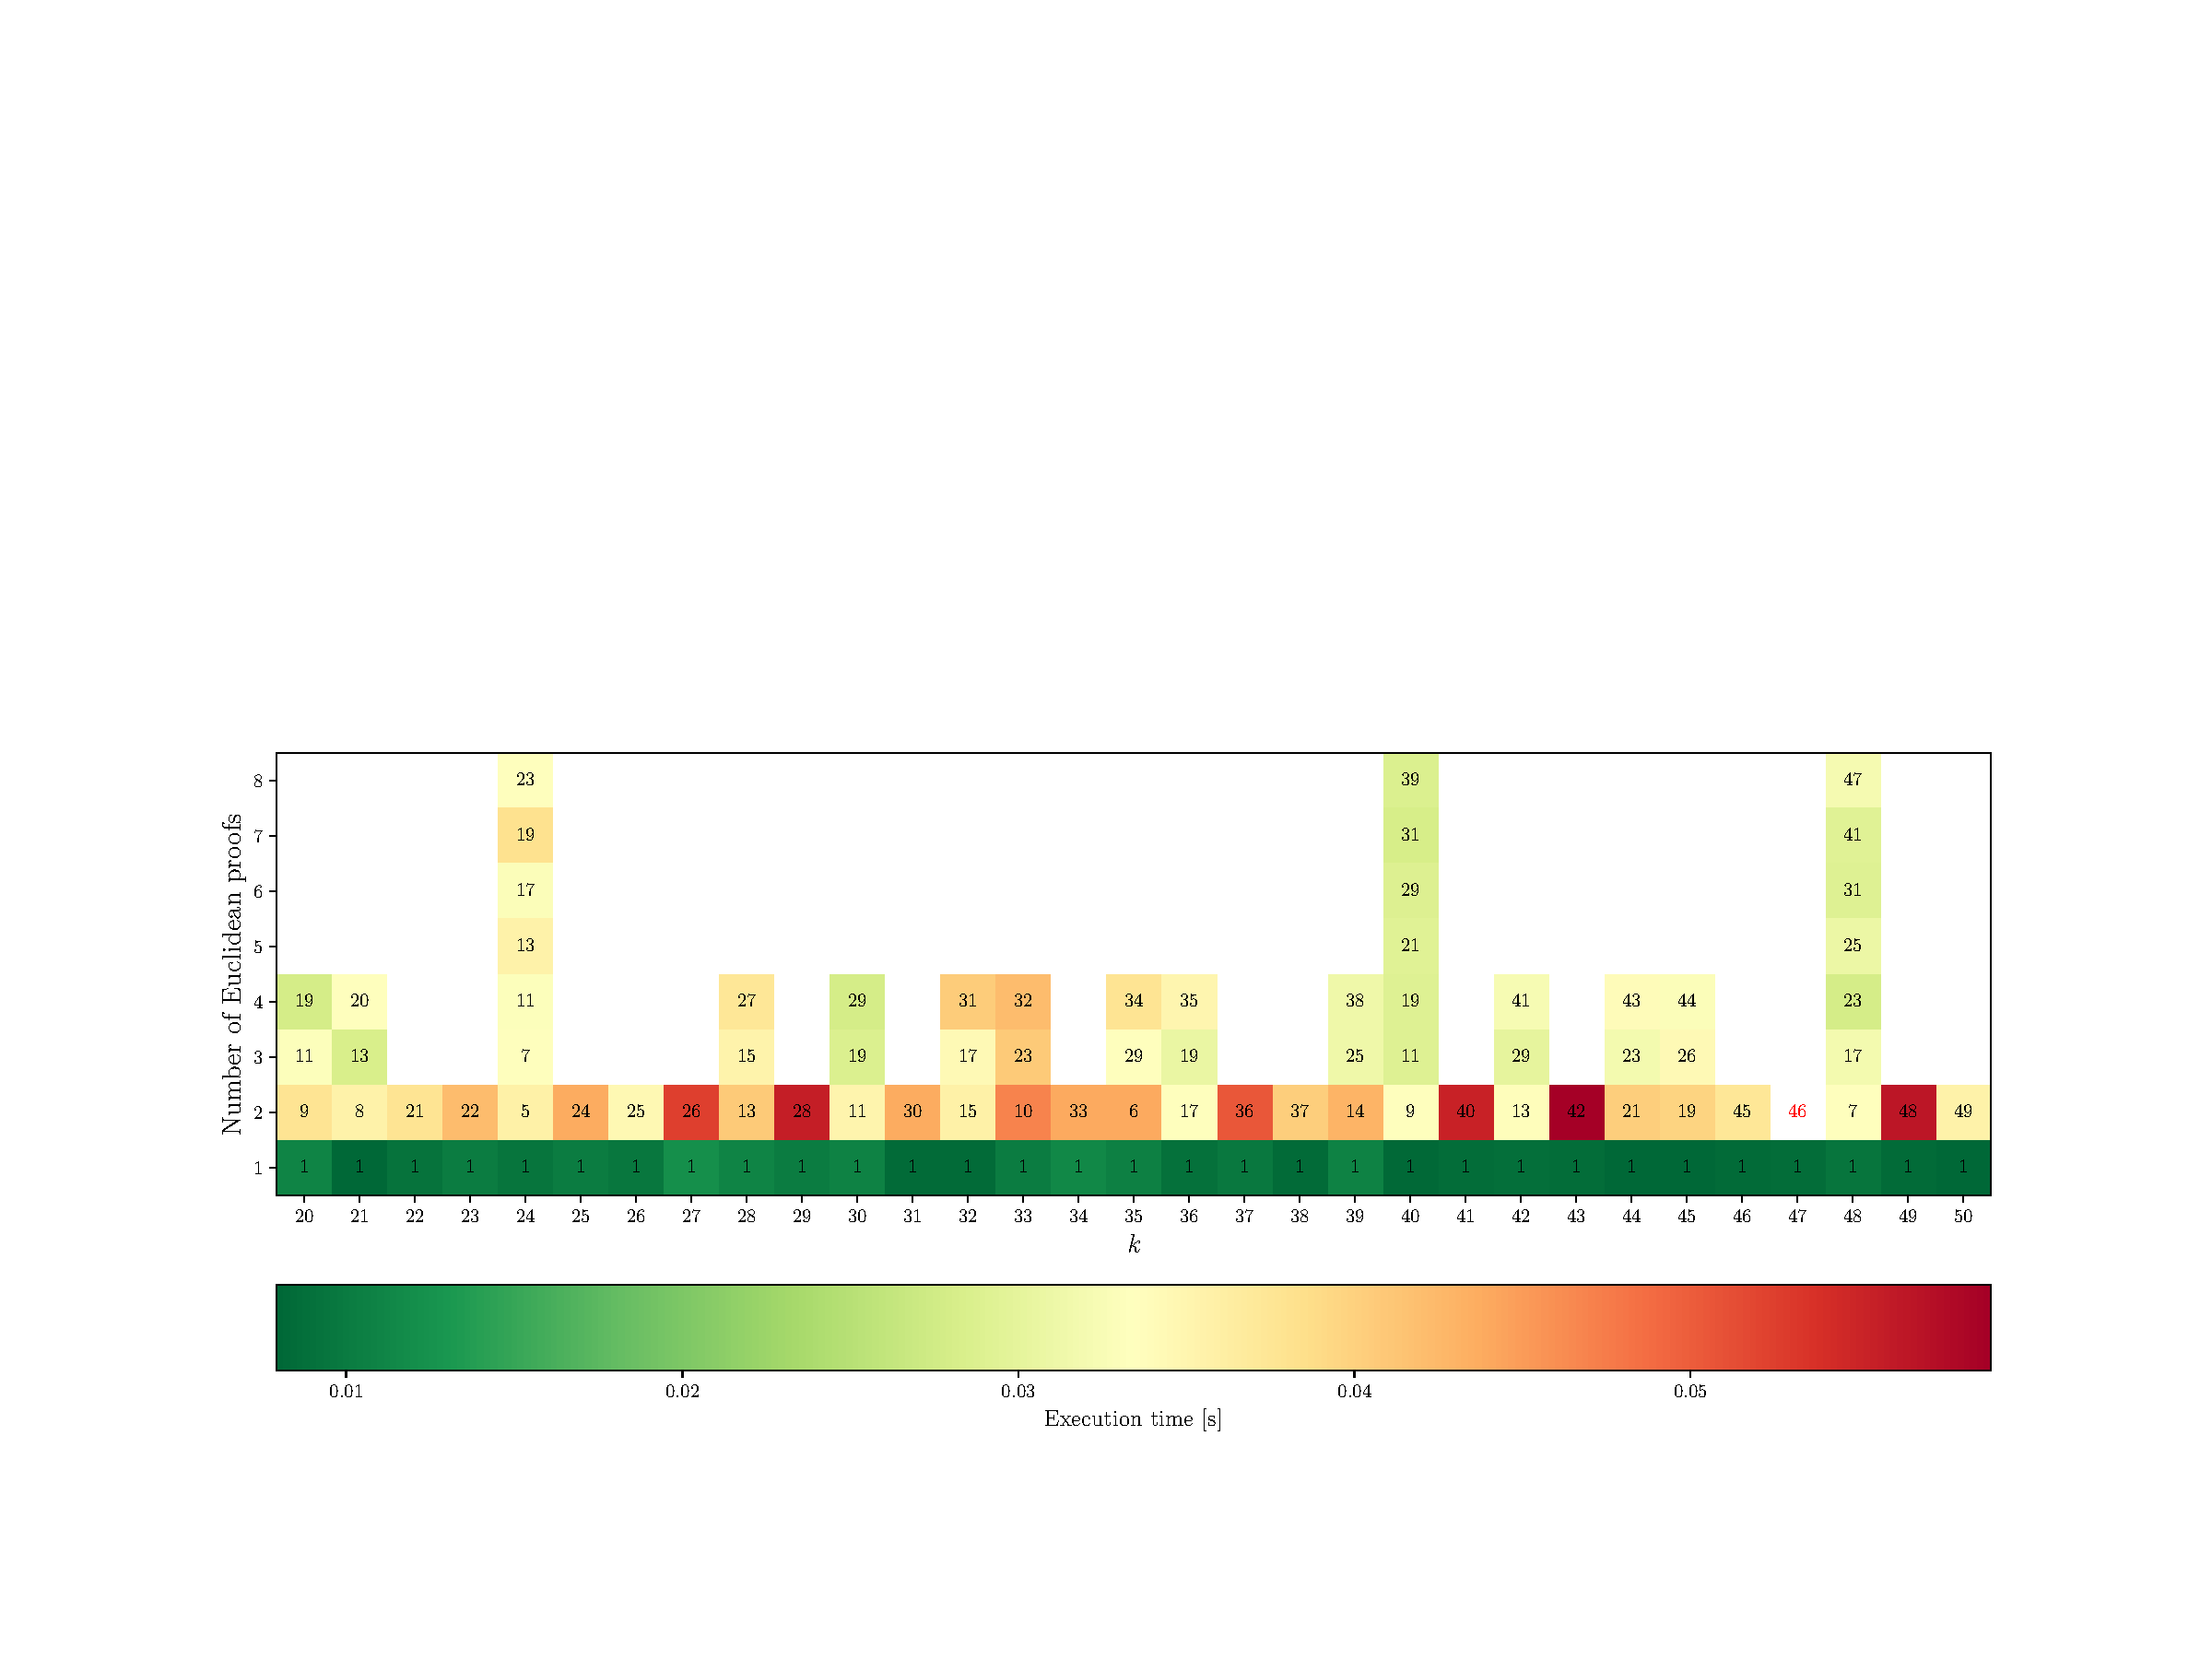
\includegraphics[width=\textwidth]{Images/running_times_20_50.eps}
	\caption{Values of $k$ and $\ell$ that satisfy $\ell^2\equiv 1 \pmod{k}$, for $k\in[20,50]$. The horizontal axis indicates the value of $k$, while the vertical axis accumulates one box for every residue class satisfying $\ell^2\equiv 1 \pmod{k}$ (the corresponding value of $\ell \bmod{k}$ is written inside the box). Observe that the number of possible Euclidean proofs (the vertical axis) is always a power of $2$, as we deduced in \cref{sec:sizeEuc}. Each box is coloured in correspondence to the execution time of the code of the arithmetic progression $\equiv\ell\pmod{k}$. If it exceeds the threshold, the corresponding value of $\ell$ is written in red within a white box.} 
	\label{fig:colouredmatrix}
\end{sidewaysfigure}

\begin{sidewaysfigure}
	\centering
	\vspace*{-3in}
	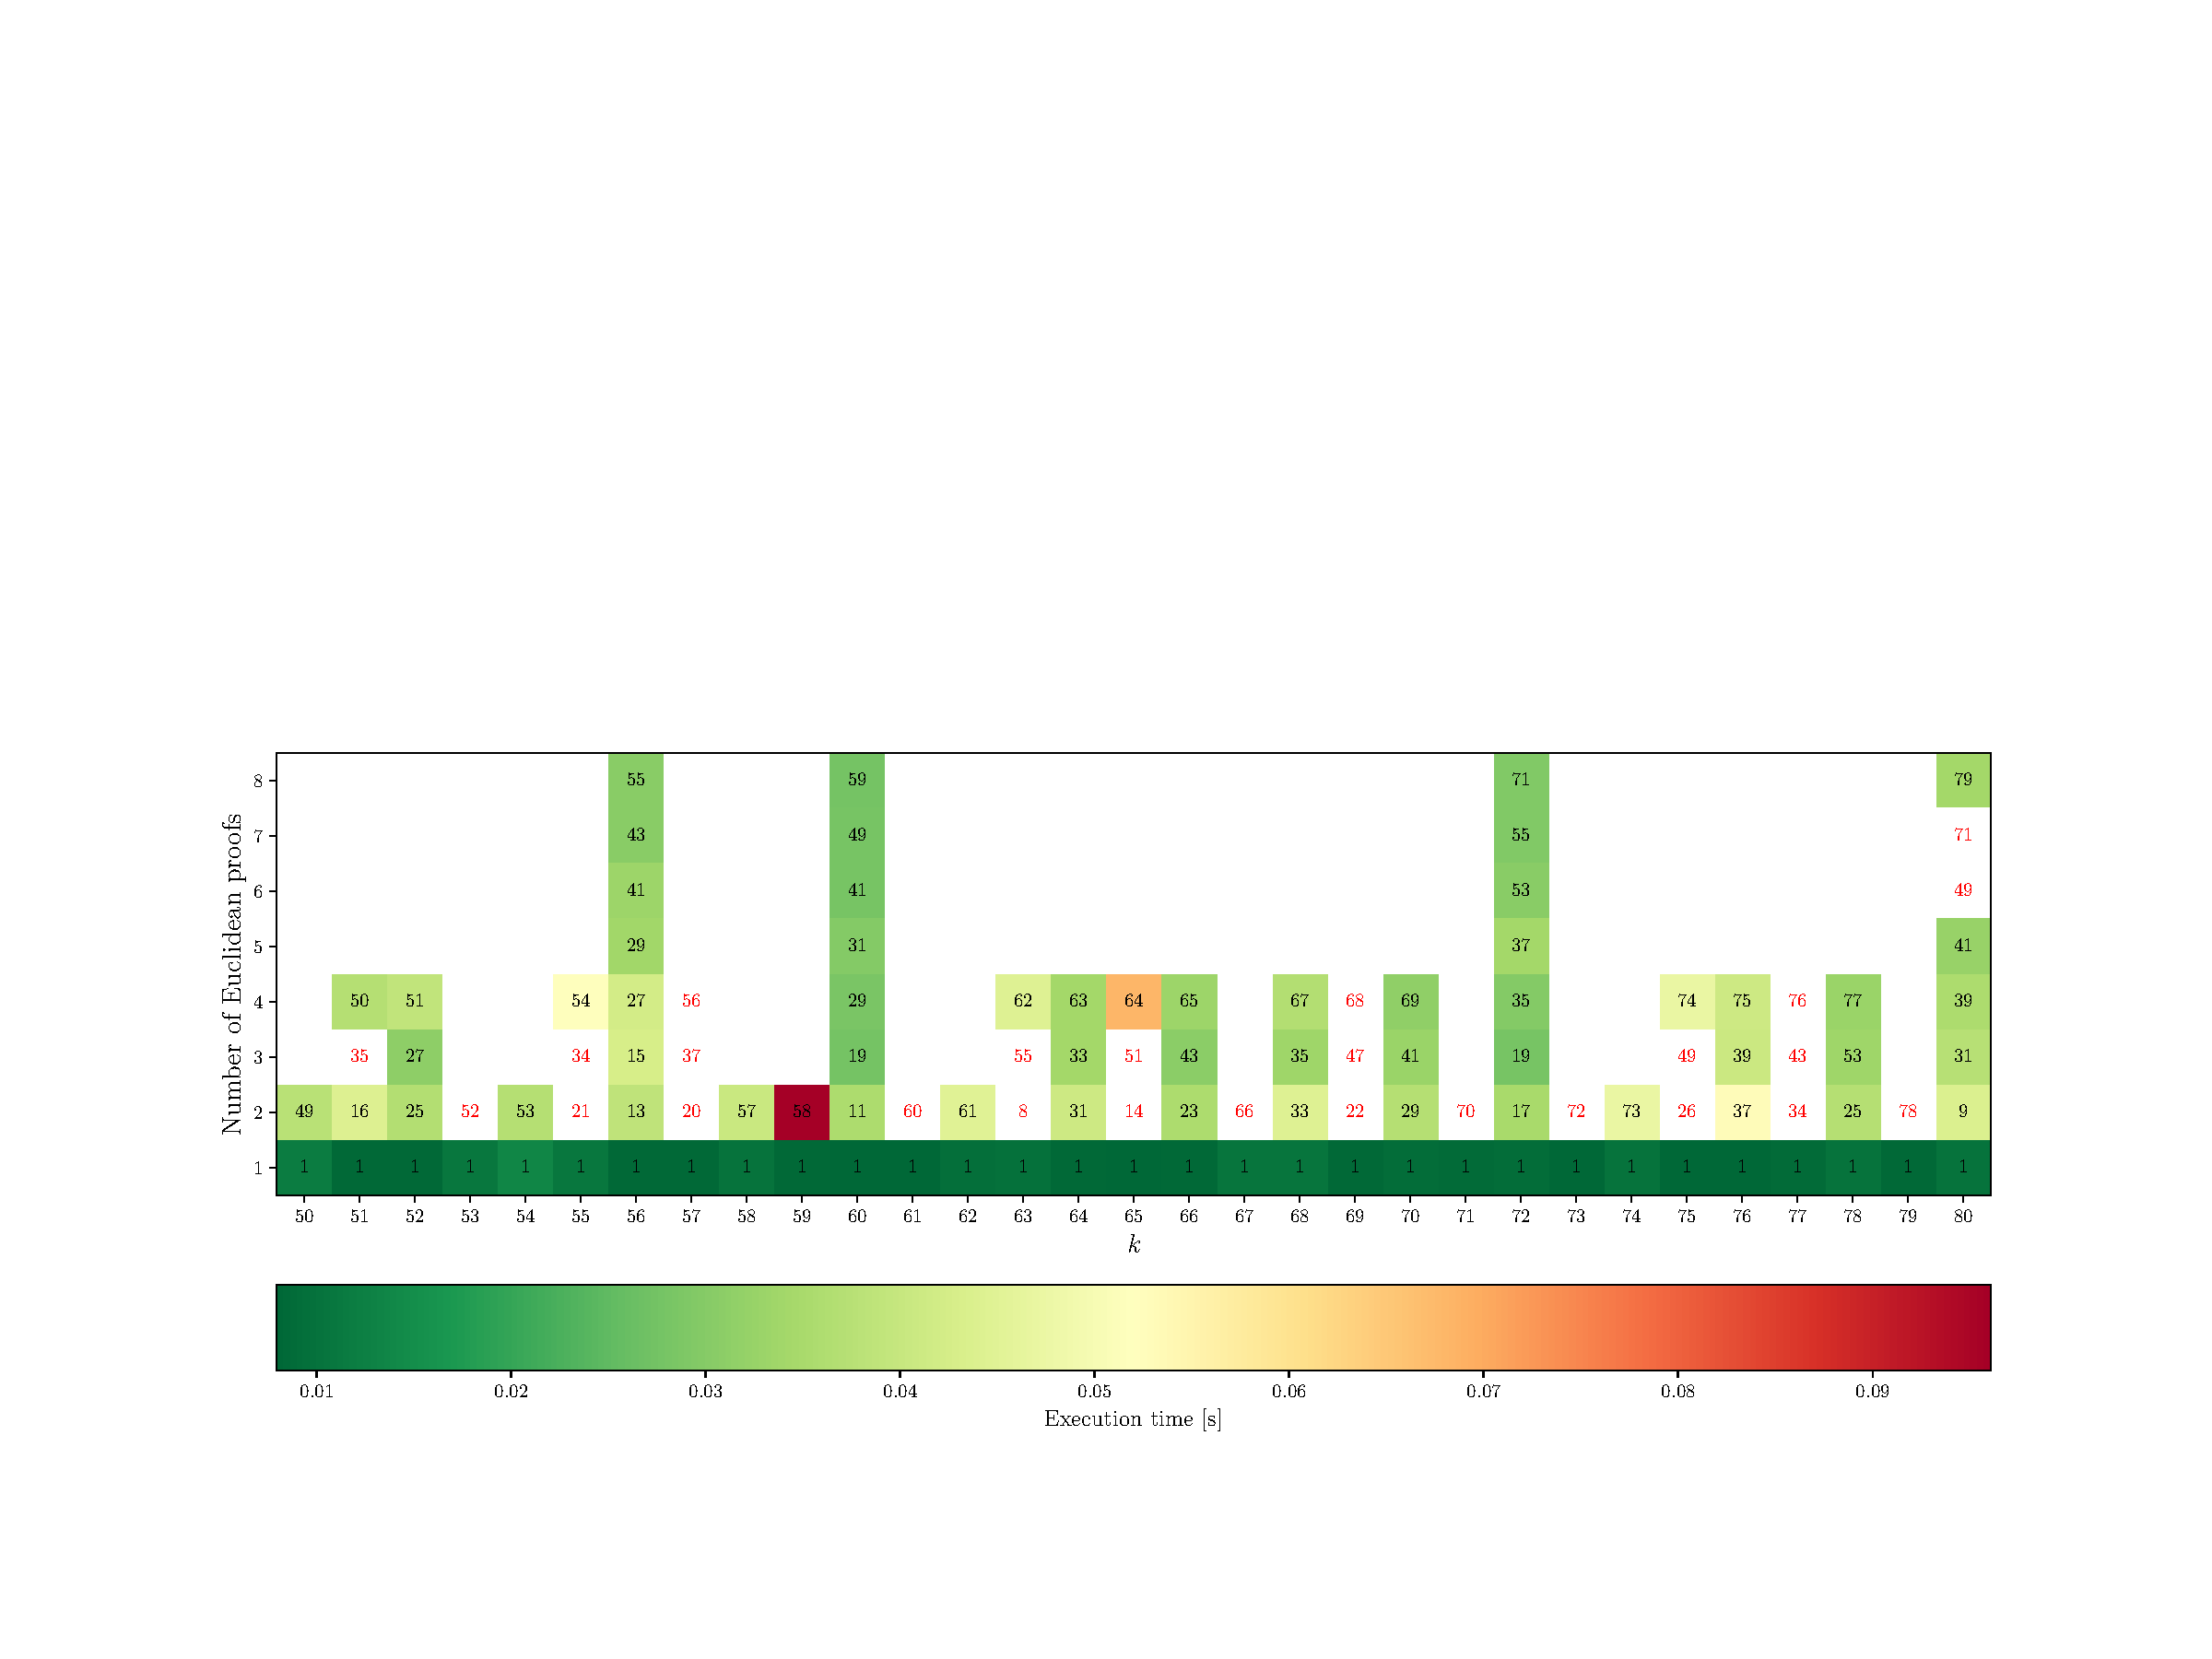
\includegraphics[width=\textwidth]{Images/running_times_50_80.eps}
	\caption{Values of $k$ and $\ell$ that satisfy $\ell^2\equiv 1 \pmod{k}$, for $k\in[50,80]$. The horizontal axis indicates the value of $k$, while the vertical axis accumulates one box for every residue class satisfying $\ell^2\equiv 1 \pmod{k}$ (the corresponding value of $\ell \bmod{k}$ is written inside the box). Observe that the number of possible Euclidean proofs (the vertical axis) is always a power of $2$, as we deduced in \cref{sec:sizeEuc}. Each box is coloured in correspondence to the execution time of the code of the arithmetic progression $\equiv\ell\pmod{k}$. If it exceeds the threshold, the corresponding value of $\ell$ is written in red within a white box.} 
	\label{fig:colouredmatrix2}
\end{sidewaysfigure}

%\begin{figure}[H]
%\begin{center}
%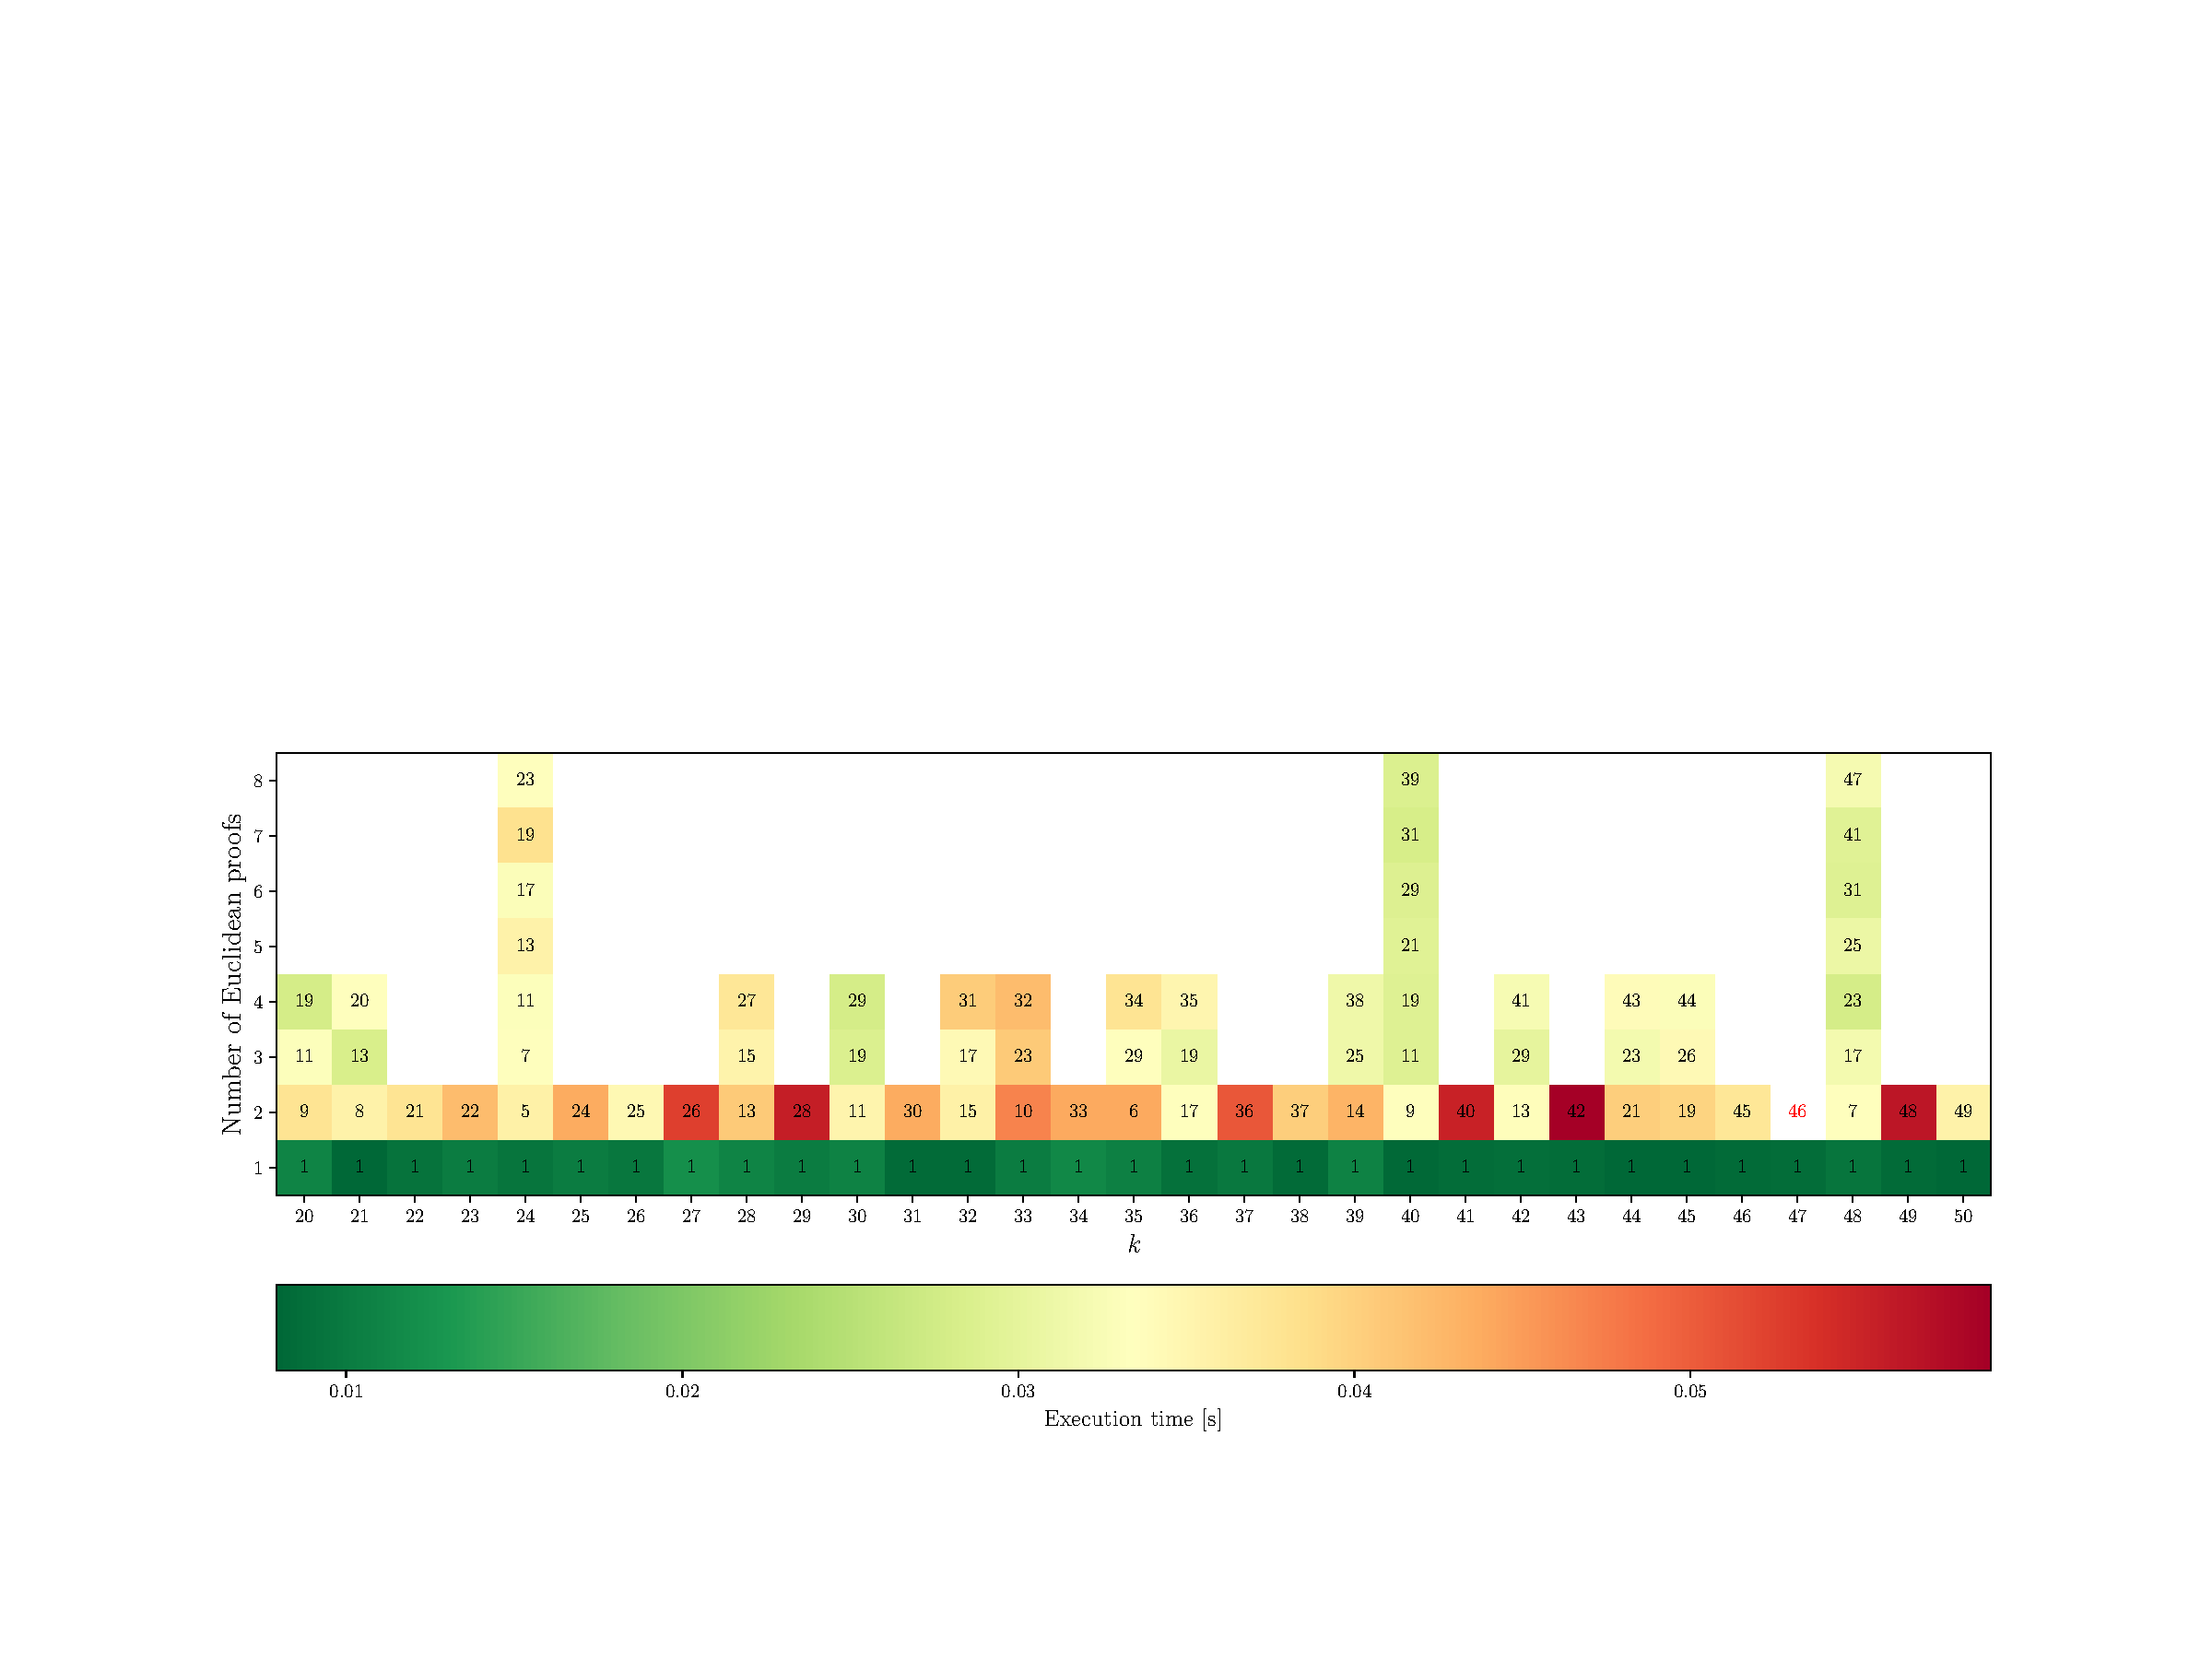
\includegraphics[width=\textwidth]{Images/running_times_20_50.png}
%\caption{Residue classes of $k\in[20,50]$ that execute under the defined threshold. Their respresentative, $\ell$, is %written in the box, which is coluored in correspondance to its execution time. If the execution of the proof of the %arithmetic progression $\equiv\ell\pmod{k}$ exceeds the threshold, the value $\ell$ is given in red. %\textcolor{red}{posar plots de varis ranges de $k$ i en format eps.}}
%\label{fig:colouredmatrix}
%\end{center}
%\end{figure}

\end{document}
